\section{Dynamics of a Single Cell}
In this section the results of the numerical solutions for a single cell
using the three models presented above are discussed. All results were
obtained with a simple Forward-Euler scheme.

\subsection{Hodgkin \& Huxley}
The equations were integrated for \SI{10}{\milli\second} with a time step
$\Delta{t}=\SI{.01}{\milli\second}$ (\ie~1000 integrations steps) and an
initial potential $V_0=\SI{-7}{\milli\volt}$.

\begin{figure}[h]
    \centering
    \begin{subfigure}[h]{.3\textwidth}
        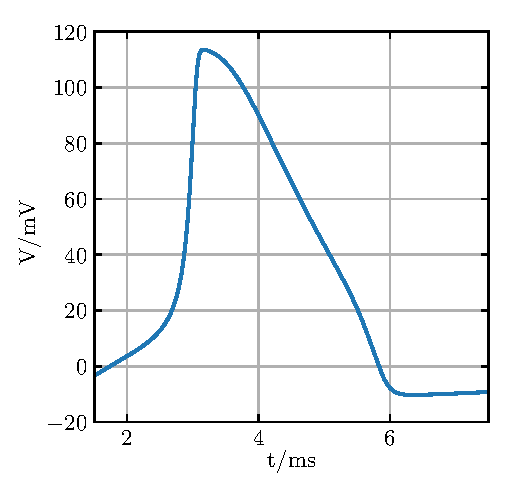
\includegraphics[width=\textwidth]{hh52-10ms-V}
        \label{fig:hh1V}
        \caption{Potential}
    \end{subfigure}
    \begin{subfigure}[h]{.3\textwidth}
        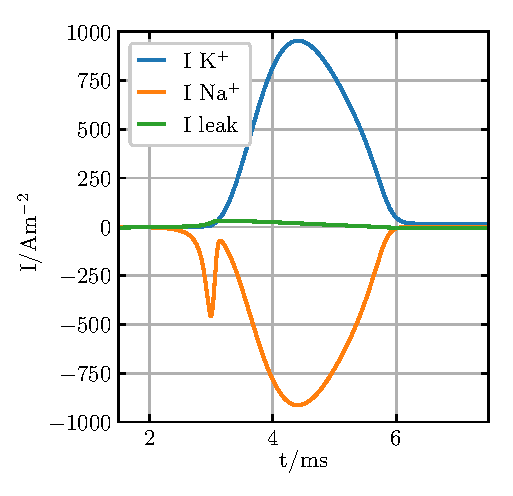
\includegraphics[width=\textwidth]{hh52-10ms-I}
        \label{fig:hh1I}
        \caption{Current Densities}
    \end{subfigure}
    \begin{subfigure}[h]{.3\textwidth}
        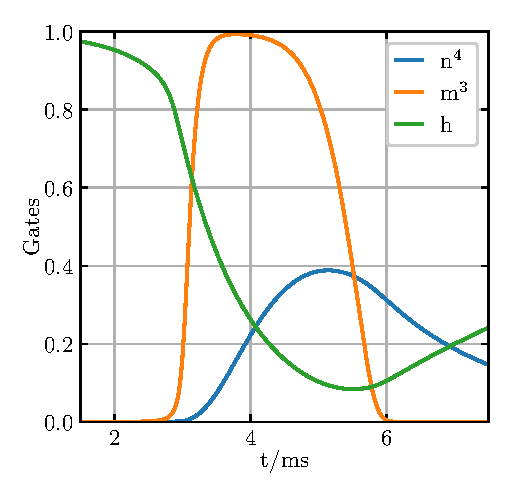
\includegraphics[width=\textwidth]{hh52-10ms-Gates}
        \label{fig:hh1Gates}
        \caption{Gating Variables}
    \end{subfigure}
    \caption{Results}
\end{figure}


% vim: set ff=unix tw=79 sw=4 ts=4 et ic ai :
